\chapter{Stream e Buffer}
\label{cap:stream_buffer}

\section*{Obiettivi di apprendimento}
Al termine di questo capitolo sarai in grado di:
\begin{itemize}
    \item Comprendere il concetto di stream in Java
    \item Utilizzare FileInputStream e FileOutputStream per operazioni su file binari
    \item Lavorare con BufferedReader e BufferedWriter per file di testo
    \item Gestire correttamente le risorse con try-with-resources
    \item Applicare le best practices nella gestione di file
\end{itemize}

\section{Introduzione agli stream}

In Java, uno \textbf{stream} (flusso) è una sequenza di dati che può essere letta o scritta. Gli stream forniscono un modo uniforme per lavorare con diverse sorgenti e destinazioni di dati: file, connessioni di rete, array in memoria, ecc.

Esistono due tipi principali di stream:

\begin{itemize}
    \item \textbf{Stream di byte} (byte streams): lavorano con dati binari, un byte alla volta. Sono le classi che terminano con \texttt{InputStream} o \texttt{OutputStream}.

    \item \textbf{Stream di caratteri} (character streams): lavorano con dati testuali, gestendo automaticamente la codifica dei caratteri. Sono le classi che terminano con \texttt{Reader} o \texttt{Writer}.
\end{itemize}

\begin{nota}
Gli stream di byte sono più versatili e possono gestire qualsiasi tipo di file, ma per file di testo è preferibile usare stream di caratteri che gestiscono correttamente encoding come UTF-8.
\end{nota}

\subsection{Esempio 1: Concetto di stream}

Immagina uno stream come un tubo attraverso cui scorrono i dati. Per leggere da un file, apri uno stream di input che porta i dati dal file al tuo programma. Per scrivere, apri uno stream di output che porta i dati dal programma al file.

\begin{lstlisting}
import java.io.FileInputStream;
import java.io.IOException;

public class StreamBasico {
    public static void main(String[] args) {
        // Apriamo uno stream per leggere dal file
        try {
            FileInputStream fis = new FileInputStream("dati.txt");

            // Leggiamo un byte alla volta
            int byteData = fis.read();

            System.out.println("Primo byte letto: " + byteData);

            // Chiudiamo lo stream
            fis.close();
        } catch (IOException e) {
            System.out.println("Errore: " + e.getMessage());
        }
    }
}
\end{lstlisting}

\subsection{Analisi del codice}

Questo esempio introduce il concetto fondamentale di stream come canale di comunicazione con file esterni. Il metodo \texttt{fis.read()} dell'oggetto \texttt{FileInputStream} restituisce un singolo byte letto dal file, rappresentato come intero (range 0-255). Quando non ci sono più dati da leggere, il metodo \texttt{fis.read()} restituisce -1.

\textbf{Perché questo approccio?} L'utilizzo di stream permette di astrarre il meccanismo di lettura: che si tratti di file su disco, dati dalla rete o altre sorgenti, l'interfaccia rimane uniforme. Tuttavia, leggere un byte alla volta è estremamente inefficiente per file di grandi dimensioni.

\textbf{Quando usare FileInputStream?} Questo pattern è adatto per file binari di piccole dimensioni o quando si necessita di controllo a basso livello sui byte. Per file di testo, è preferibile usare stream di caratteri (Reader/Writer).

\textbf{Nota sulla gestione delle risorse:} Questo esempio mostra una chiusura esplicita dello stream con il metodo \texttt{fis.close()}. Nelle sezioni successive vedremo il pattern try-with-resources che automatizza questo processo critico.

\begin{figure}[h]
\centering
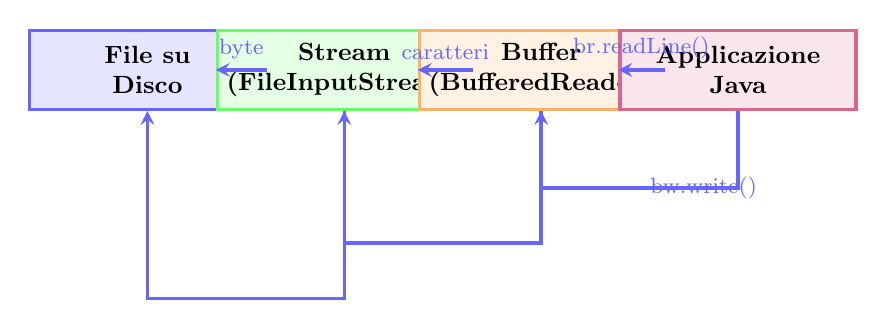
\begin{tikzpicture}[
    node distance=2.5cm,
    block/.style={
        rectangle,
        draw=blue!60,
        fill=blue!10,
        very thick,
        minimum width=3cm,
        minimum height=1cm,
        align=center,
        font=\small\bfseries
    },
    arrow/.style={
        ->,
        >=stealth,
        very thick,
        blue!60
    }
]

% Blocchi del flusso
\node[block] (file) {File su\\Disco};
\node[block, right of=file, fill=green!10, draw=green!60] (stream) {Stream\\(FileInputStream)};
\node[block, right of=stream, fill=orange!10, draw=orange!60] (buffer) {Buffer\\(BufferedReader)};
\node[block, right of=buffer, fill=purple!10, draw=purple!60] (app) {Applicazione\\Java};

% Frecce
\draw[arrow] (file) -- (stream) node[midway, above, font=\footnotesize] {byte};
\draw[arrow] (stream) -- (buffer) node[midway, above, font=\footnotesize] {caratteri};
\draw[arrow] (buffer) -- (app) node[midway, above, font=\footnotesize] {br.readLine()};

% Frecce di ritorno (output)
\draw[arrow] (app) -- +(0,-1.5) -| (buffer) node[near start, right, font=\footnotesize] {bw.write()};
\draw[arrow] (buffer) -- +(0,-2.2) -| (stream);
\draw[arrow] (stream) -- +(0,-2.9) -| (file);

\end{tikzpicture}
\caption{Flusso di dati tra file, stream, buffer e applicazione. I dati viaggiano dal disco all'applicazione attraverso stream e buffer, ottimizzando le performance}
\label{fig:flusso_stream}
\end{figure}

\section{Input e Output Stream}

La gerarchia delle classi per gestire gli stream in Java è organizzata attorno a quattro classi astratte principali:

\begin{itemize}
    \item \texttt{InputStream}: classe base per leggere byte
    \item \texttt{OutputStream}: classe base per scrivere byte
    \item \texttt{Reader}: classe base per leggere caratteri
    \item \texttt{Writer}: classe base per scrivere caratteri
\end{itemize}

Da queste classi derivano implementazioni concrete come \texttt{FileInputStream}, \texttt{FileOutputStream}, \texttt{FileReader}, \texttt{FileWriter}, ecc.

\subsection{Esempio 2: Lettura byte per byte}

\begin{lstlisting}
import java.io.FileInputStream;
import java.io.IOException;

public class LeggiFile {
    public static void main(String[] args) {
        FileInputStream fis = null;

        try {
            fis = new FileInputStream("input.dat");
            int byteData;

            // fis.read() restituisce -1 quando raggiunge la fine del file
            while ((byteData = fis.read()) != -1) {
                System.out.print((char) byteData);
            }
        } catch (IOException e) {
            System.out.println("Errore nella lettura: " + e.getMessage());
        } finally {
            // Importante: chiudere sempre lo stream
            try {
                if (fis != null) {
                    fis.close();
                }
            } catch (IOException e) {
                System.out.println("Errore nella chiusura: " + e.getMessage());
            }
        }
    }
}
\end{lstlisting}

\subsection{Analisi del codice}

Questo esempio dimostra il pattern classico di lettura completa di un file utilizzando un ciclo while che continua finché il metodo \texttt{fis.read()} non restituisce -1 (indicatore di fine file, EOF - End Of File). Il cast \texttt{(char)} converte ogni byte in carattere per la visualizzazione.

\textbf{Perché il blocco finally?} La gestione della chiusura nel blocco \texttt{finally} garantisce che lo stream venga liberato anche in caso di eccezioni durante la lettura. Il controllo \texttt{if (fis != null)} previene \texttt{NullPointerException} se l'apertura dello stream fallisce.

\textbf{Pattern try-finally:} Questa tecnica, pur essendo corretta, è verbosa e soggetta a errori. Il programmatore deve ricordarsi di gestire due possibili eccezioni: una durante l'operazione di I/O e una durante la chiusura. Questo pattern è stato semplificato in Java 7 con try-with-resources.

\textbf{Limitazioni:} Leggere byte per byte è molto inefficiente. Ogni chiamata al metodo \texttt{fis.read()} comporta un accesso al disco. Per un file di 1 MB servirebbero circa 1.000.000 di operazioni di I/O, rendendo il processo estremamente lento.

\begin{errore}
Dimenticare di chiudere uno stream può causare memory leak e file bloccati. Gli stream tengono aperte risorse di sistema che devono essere liberate esplicitamente.
\end{errore}

\section{FileInputStream e FileOutputStream}

\texttt{FileInputStream} e \texttt{FileOutputStream} sono le classi più semplici per lavorare con file. Operano a livello di byte e sono adatte per file binari (immagini, audio, video) ma anche per file di testo.

\subsection{Metodi principali di FileInputStream}

\begin{itemize}
    \item \texttt{stream.read()}: legge un singolo byte e lo restituisce come int (0-255), oppure -1 se fine file
    \item \texttt{stream.read(byte[] b)}: legge byte e li memorizza nell'array, restituisce il numero di byte letti
    \item \texttt{stream.close()}: chiude lo stream e rilascia le risorse
    \item \texttt{stream.available()}: restituisce una stima dei byte disponibili per la lettura
\end{itemize}

\subsection{Metodi principali di FileOutputStream}

\begin{itemize}
    \item \texttt{stream.write(int b)}: scrive un singolo byte
    \item \texttt{stream.write(byte[] b)}: scrive un array di byte
    \item \texttt{stream.flush()}: forza la scrittura immediata dei dati bufferizzati
    \item \texttt{stream.close()}: chiude lo stream
\end{itemize}

\subsection{Esempio 3: Copia di un file}

\begin{lstlisting}
import java.io.FileInputStream;
import java.io.FileOutputStream;
import java.io.IOException;

public class CopiaFile {
    public static void main(String[] args) {
        FileInputStream sorgente = null;
        FileOutputStream destinazione = null;

        try {
            sorgente = new FileInputStream("originale.jpg");
            destinazione = new FileOutputStream("copia.jpg");

            // Array buffer per lettura/scrittura più efficiente
            byte[] buffer = new byte[1024]; // 1 KB alla volta
            int byteLetti;

            // Leggi e scrivi in blocchi
            while ((byteLetti = sorgente.read(buffer)) != -1) {
                destinazione.write(buffer, 0, byteLetti);
            }

            System.out.println("File copiato con successo!");

        } catch (IOException e) {
            System.out.println("Errore: " + e.getMessage());
        } finally {
            try {
                if (sorgente != null) sorgente.close();
                if (destinazione != null) destinazione.close();
            } catch (IOException e) {
                System.out.println("Errore chiusura: " + e.getMessage());
            }
        }
    }
}
\end{lstlisting}

\subsection{Analisi del codice}

Questo esempio implementa una funzionalità di copia file utilizzando un buffer intermedio per ottimizzare le performance. La tecnica del buffering manuale riduce drasticamente gli accessi al disco rispetto alla lettura byte-per-byte.

\textbf{Come funziona il buffer?} L'array \texttt{byte[] buffer = new byte[1024]} crea uno spazio in memoria di 1 KB. Il metodo \texttt{sorgente.read(buffer)} legge fino a 1024 byte dal file sorgente e li memorizza nell'array, restituendo il numero effettivo di byte letti. Questo approccio riduce 1024 chiamate di sistema a una singola operazione.

\textbf{Perché destinazione.write(buffer, 0, byteLetti)?} Nell'ultima iterazione, il file potrebbe non riempire completamente il buffer. Il parametro \texttt{byteLetti} indica quanti byte sono stati effettivamente letti, evitando di scrivere dati spazzatura oltre la fine del file reale.

\textbf{Scelta della dimensione del buffer:} 1 KB è un buon compromesso tra uso di memoria e performance. Buffer più grandi (4-8 KB) possono migliorare ulteriormente la velocità, ma oltre certi limiti i benefici diventano marginali. Per file molto grandi, buffer di 8-16 KB sono ottimali.

\textbf{Applicabilità:} Questo pattern funziona con qualsiasi tipo di file (binario o testo) perché opera a livello di byte grezzo, preservando perfettamente la struttura del file originale.

\begin{nota}
Usare un buffer (array di byte) invece di leggere un byte alla volta migliora drasticamente le performance, riducendo il numero di accessi al disco.
\end{nota}

\subsection{Esempio 4: Scrittura su file}

\begin{lstlisting}
import java.io.FileOutputStream;
import java.io.IOException;

public class ScriviFile {
    public static void main(String[] args) {
        try {
            FileOutputStream fos = new FileOutputStream("output.txt");

            String testo = "Ciao mondo da Java!";
            byte[] dati = testo.getBytes(); // Converte String in byte[]

            fos.write(dati);
            fos.close();

            System.out.println("Scrittura completata!");

        } catch (IOException e) {
            System.out.println("Errore: " + e.getMessage());
        }
    }
}
\end{lstlisting}

\subsection{Analisi del codice}

Questo esempio mostra come scrivere dati testuali su file utilizzando stream di byte. Il metodo \texttt{testo.getBytes()} dell'oggetto \texttt{String} converte una stringa Java in un array di byte utilizzando l'encoding di default della piattaforma (tipicamente UTF-8 su sistemi moderni).

\textbf{Conversione String-Byte:} Le stringhe in Java sono sequenze di caratteri Unicode (16 bit ciascuno), mentre i file memorizzano byte (8 bit). La conversione tramite il metodo \texttt{testo.getBytes()} applica un encoding per rappresentare i caratteri come sequenze di byte. Per controllare esplicitamente l'encoding, si può usare il metodo \texttt{testo.getBytes("UTF-8")}.

\textbf{Quando usare FileOutputStream per testo?} Questo approccio è adatto per scritture semplici e veloci, ma presenta limitazioni: non gestisce automaticamente le newline in modo portabile tra sistemi operativi e non offre buffering integrato. Per operazioni testuali complesse, \texttt{BufferedWriter} è preferibile.

\textbf{Modalità di scrittura:} Di default, \texttt{FileOutputStream} crea un nuovo file o sovrascrive quello esistente. La modalità "append" (aggiunta in coda) preserva il contenuto esistente, utile per file di log o quando si vogliono aggiungere dati progressivamente.

\begin{attenzione}
Per default, \texttt{FileOutputStream} sovrascrive il file esistente. Per aggiungere dati in coda, usa il costruttore con secondo parametro true: \\
\texttt{new FileOutputStream("file.txt", true)}
\end{attenzione}

\section{BufferedReader e BufferedWriter}

Per lavorare con file di testo, le classi \texttt{BufferedReader} e \texttt{BufferedWriter} sono più efficienti e comode. Il buffering interno riduce gli accessi al disco e fornisce metodi utili come \texttt{br.readLine()} (dove \texttt{br} è un oggetto \texttt{BufferedReader}) per leggere righe intere.

\subsection{Vantaggi del buffering}

Un buffer è una zona di memoria temporanea che accumula dati prima di leggerli/scriverli effettivamente. Invece di accedere al disco per ogni singolo carattere, si legge/scrive in blocchi, riducendo drasticamente i tempi di I/O.

\subsection{Esempio 5: Lettura di file di testo riga per riga}

\begin{lstlisting}
import java.io.BufferedReader;
import java.io.FileReader;
import java.io.IOException;

public class LeggiTestoRighe {
    public static void main(String[] args) {
        BufferedReader br = null;

        try {
            // FileReader legge caratteri, BufferedReader aggiunge buffering
            br = new BufferedReader(new FileReader("testo.txt"));

            String riga;
            int numeroRiga = 1;

            // br.readLine() legge una riga intera e restituisce null a fine file
            while ((riga = br.readLine()) != null) {
                System.out.println(numeroRiga + ": " + riga);
                numeroRiga++;
            }

        } catch (IOException e) {
            System.out.println("Errore: " + e.getMessage());
        } finally {
            try {
                if (br != null) br.close();
            } catch (IOException e) {
                System.out.println("Errore chiusura: " + e.getMessage());
            }
        }
    }
}
\end{lstlisting}

\subsection{Analisi del codice}

Questo esempio mostra l'approccio moderno e raccomandato per leggere file di testo in Java. La combinazione \texttt{FileReader} + \texttt{BufferedReader} crea una pipeline efficiente: \texttt{FileReader} gestisce la conversione byte-caratteri, mentre \texttt{BufferedReader} aggiunge buffering e il metodo \texttt{br.readLine()}.

\textbf{Perché il decorator pattern?} Java usa il pattern Decorator per comporre funzionalità. \texttt{BufferedReader} "decora" \texttt{FileReader} aggiungendo buffering. Questo design modulare permette di combinare diverse capacità: si potrebbe aggiungere ulteriore compressione, cifratura, ecc., semplicemente impilando più decorator.

\textbf{Il metodo br.readLine():} Questo metodo dell'oggetto \texttt{BufferedReader} legge caratteri fino al prossimo separatore di riga (\texttt{\textbackslash n}, \texttt{\textbackslash r\textbackslash n}, o \texttt{\textbackslash r}) e restituisce la stringa senza il separatore. Quando raggiunge la fine del file, il metodo \texttt{br.readLine()} restituisce \texttt{null} (non stringa vuota).

\textbf{Vantaggi del buffering automatico:} Internamente, \texttt{BufferedReader} legge blocchi di caratteri (default 8192 caratteri) e li memorizza. Le chiamate successive a \texttt{br.readLine()} attingono da questo buffer interno, riducendo drasticamente le chiamate di sistema.

\textbf{Gestione encoding:} \texttt{FileReader} usa l'encoding di default del sistema. Per specificare un encoding (es. UTF-8), usa invece: \\
\texttt{new BufferedReader(new InputStreamReader(new FileInputStream("file.txt"), "UTF-8"))}

\subsection{Esempio 6: Scrittura su file di testo con BufferedWriter}

\begin{lstlisting}
import java.io.BufferedWriter;
import java.io.FileWriter;
import java.io.IOException;

public class ScriviTestoBuffer {
    public static void main(String[] args) {
        try {
            BufferedWriter bw = new BufferedWriter(
                new FileWriter("output.txt")
            );

            // Scriviamo diverse righe
            bw.write("Prima riga di testo");
            bw.newLine(); // Aggiunge il separatore di riga corretto per l'OS
            bw.write("Seconda riga di testo");
            bw.newLine();
            bw.write("Terza riga");

            bw.close(); // Chiude e fa flush automatico

            System.out.println("File scritto con successo!");

        } catch (IOException e) {
            System.out.println("Errore: " + e.getMessage());
        }
    }
}
\end{lstlisting}

\subsection{Analisi del codice}

Questo esempio illustra la scrittura su file di testo utilizzando il buffering per ottimizzare le performance. Come per la lettura, la combinazione \texttt{FileWriter} + \texttt{BufferedWriter} crea una pipeline: \texttt{FileWriter} gestisce la conversione caratteri-byte, mentre \texttt{BufferedWriter} aggiunge buffering.

\textbf{Il metodo bw.newLine():} Questo metodo dell'oggetto \texttt{BufferedWriter} è fondamentale per la portabilità del codice. Scrive il separatore di riga appropriato per il sistema operativo corrente: \texttt{\textbackslash r\textbackslash n} su Windows, \texttt{\textbackslash n} su Unix/Linux/macOS. Hardcodare \texttt{"\textbackslash n"} creerebbe file non conformi su Windows.

\textbf{Buffering in scrittura:} I dati non vengono scritti immediatamente su disco ma accumulati in un buffer interno (default 8192 caratteri). La scrittura fisica avviene quando: (1) il buffer si riempie, (2) si chiama il metodo \texttt{bw.flush()}, (3) si chiude lo stream. Questo riduce drasticamente le operazioni di I/O.

\textbf{Importanza di bw.close():} La chiusura dello stream è critica perché: (1) forza il flush dei dati bufferizzati, (2) libera le risorse di sistema, (3) rende disponibile il file ad altri processi. Senza il metodo \texttt{bw.close()}, gli ultimi dati potrebbero non essere scritti su disco.

\textbf{Alternative moderne:} Da Java 11 è disponibile anche \texttt{Files.writeString(Path, String)} per scritture semplici one-liner.

\begin{nota}
Il metodo \texttt{bw.newLine()} dell'oggetto \texttt{BufferedWriter} è preferibile a scrivere manualmente \texttt{"\textbackslash n"} perché usa il separatore di riga corretto per il sistema operativo (Windows usa \texttt{"\textbackslash r\textbackslash n"}, Unix/Linux usa \texttt{"\textbackslash n"}).
\end{nota}

\section{File di Testo vs File di Oggetti (Serializzazione)}

Finora abbiamo lavorato principalmente con file di testo, dove i dati sono memorizzati in formato leggibile. Esiste però un'alternativa potente per salvare dati strutturati: la \textbf{serializzazione degli oggetti}. Questa sezione esplora le differenze tra questi due approcci e quando usare ciascuno.

\subsection{File di Testo}

I \textbf{file di testo} memorizzano dati in formato leggibile da esseri umani, utilizzando encoding come UTF-8, ASCII, ISO-8859-1, ecc. Ogni carattere è rappresentato da uno o più byte secondo lo schema di codifica scelto.

\subsubsection{Caratteristiche dei file di testo}

\begin{itemize}
    \item \textbf{Leggibilità umana:} Possono essere aperti e modificati con qualsiasi editor di testo
    \item \textbf{Portabilità:} Funzionano su qualsiasi piattaforma, indipendentemente dal linguaggio
    \item \textbf{Interoperabilità:} Facili da processare con script, tool Unix, Excel, ecc.
    \item \textbf{Debugging semplice:} È possibile ispezionare direttamente il contenuto
    \item \textbf{Separatori di riga:} Gestione di newline (\texttt{\textbackslash n}, \texttt{\textbackslash r\textbackslash n})
    \item \textbf{Encoding:} Necessità di specificare la codifica caratteri (UTF-8, ecc.)
\end{itemize}

\subsubsection{Quando usare file di testo}

I file di testo sono la scelta ideale per:

\begin{itemize}
    \item \textbf{File di configurazione:} properties, ini, yaml, json, xml
    \item \textbf{Log applicativi:} tracciamento eventi e debugging
    \item \textbf{Dati tabulari:} CSV, TSV per export verso Excel/database
    \item \textbf{Documentazione:} markdown, plain text
    \item \textbf{Scambio dati tra linguaggi diversi:} JSON, XML
    \item \textbf{Archiviazione long-term:} dati che devono essere accessibili per anni
\end{itemize}

\subsubsection{Vantaggi e svantaggi}

\begin{table}[h]
\centering
\begin{tabular}{|p{6cm}|p{6cm}|}
\hline
\textbf{Vantaggi} & \textbf{Svantaggi} \\
\hline
Leggibili e modificabili manualmente & Occupano più spazio su disco \\
\hline
Indipendenti dal linguaggio & Parsing necessario per ricostruire oggetti \\
\hline
Facili da debuggare & Performance inferiori per strutture complesse \\
\hline
Stabili nel tempo & Perdita di tipo (tutto diventa stringa) \\
\hline
Tool diffusi per elaborazione & Difficoltà con strutture annidate profonde \\
\hline
\end{tabular}
\end{table}

\subsection{File di Oggetti - Serializzazione}

La \textbf{serializzazione} è il processo di conversione di un oggetto Java in una sequenza di byte che può essere salvata su file o trasmessa in rete. Il processo inverso si chiama \textbf{deserializzazione} e ricostruisce l'oggetto originale dallo stream di byte.

\subsubsection{Cos'è la serializzazione}

La serializzazione permette di:
\begin{itemize}
    \item Salvare lo \textbf{stato completo} di un oggetto (valori di tutti i campi)
    \item Preservare la \textbf{struttura dei dati} (tipo, relazioni tra oggetti)
    \item Gestire automaticamente \textbf{grafi di oggetti} (oggetti che referenziano altri oggetti)
    \item Mantenere \textbf{l'identità degli oggetti} (se A e B puntano allo stesso oggetto C, dopo deserializzazione questa relazione è preservata)
\end{itemize}

\subsubsection{L'interfaccia Serializable}

Per rendere una classe serializzabile, è sufficiente implementare l'interfaccia marker \texttt{java.io.Serializable}:

\begin{lstlisting}
import java.io.Serializable;

public class Studente implements Serializable {
    private String nome;
    private String cognome;
    private int matricola;
    private double media;

    // Costruttori, getter, setter, toString...
}
\end{lstlisting}

\texttt{Serializable} è un'interfaccia \textbf{marker} (senza metodi) che indica alla JVM che la classe può essere serializzata. Non implementarla causa \texttt{NotSerializableException} a runtime.

\subsubsection{Come funziona la serializzazione}

Quando serializzi un oggetto, Java:

\begin{enumerate}
    \item Scrive i \textbf{metadata} della classe (nome, versione, struttura)
    \item Scrive i \textbf{valori di tutti i campi} non-transient
    \item Se un campo è un oggetto, lo \textbf{serializza ricorsivamente}
    \item Gestisce riferimenti circolari memorizzando ogni oggetto una sola volta
    \item Crea uno stream binario compatto
\end{enumerate}

Durante la deserializzazione:

\begin{enumerate}
    \item Legge i metadata e verifica la compatibilità della classe
    \item Alloca memoria per l'oggetto \textbf{senza chiamare il costruttore}
    \item Popola i campi con i valori deserializzati
    \item Ricostruisce i riferimenti tra oggetti
\end{enumerate}

\subsubsection{ObjectOutputStream e ObjectInputStream}

Java fornisce due classi specializzate per la serializzazione:

\begin{itemize}
    \item \texttt{ObjectOutputStream}: scrive oggetti su uno stream
    \item \texttt{ObjectInputStream}: legge oggetti da uno stream
\end{itemize}

Metodi principali di \texttt{ObjectOutputStream} e \texttt{ObjectInputStream}:

\begin{lstlisting}
// Scrittura
ObjectOutputStream oos = new ObjectOutputStream(
    new FileOutputStream("studenti.dat")
);
oos.writeObject(oggetto);  // Serializza e scrive l'oggetto
oos.close();

// Lettura
ObjectInputStream ois = new ObjectInputStream(
    new FileInputStream("studenti.dat")
);
Studente s = (Studente) ois.readObject();  // Legge e deserializza
ois.close();
\end{lstlisting}

\begin{figure}[h]
\centering
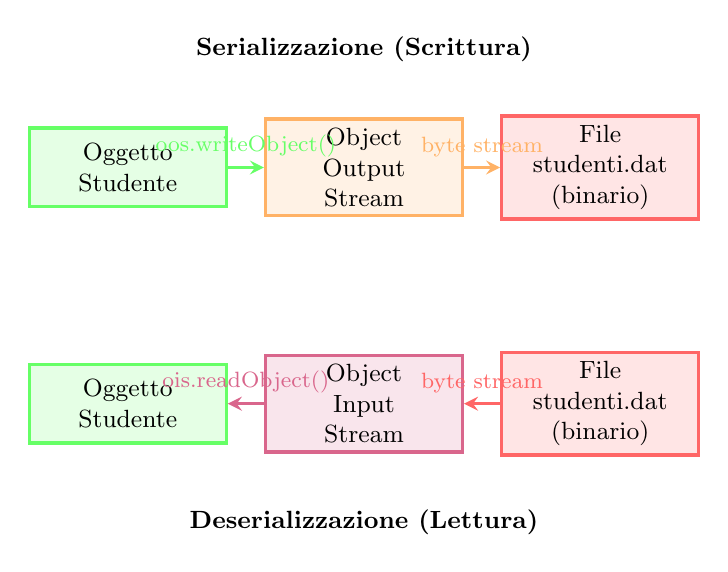
\begin{tikzpicture}[
    node distance=3cm,
    block/.style={
        rectangle,
        draw=blue!60,
        fill=blue!10,
        very thick,
        minimum width=2.5cm,
        minimum height=1cm,
        align=center,
        font=\small
    },
    arrow/.style={
        ->,
        >=stealth,
        very thick
    }
]

% Parte superiore - Scrittura (Serializzazione)
\node[block, fill=green!10, draw=green!60] (obj1) {Oggetto\\Studente};
\node[block, right of=obj1, fill=orange!10, draw=orange!60] (oos) {Object\\Output\\Stream};
\node[block, right of=oos, fill=red!10, draw=red!60] (file1) {File\\studenti.dat\\(binario)};

\draw[arrow, green!60, very thick] (obj1) -- (oos) node[midway, above, font=\footnotesize] {oos.writeObject()};
\draw[arrow, orange!60, very thick] (oos) -- (file1) node[midway, above, font=\footnotesize] {byte stream};

% Etichetta per la direzione
\node[above of=oos, node distance=1.5cm, font=\small\bfseries] {Serializzazione (Scrittura)};

% Parte inferiore - Lettura (Deserializzazione)
\node[block, fill=red!10, draw=red!60, below of=file1, node distance=3cm] (file2) {File\\studenti.dat\\(binario)};
\node[block, left of=file2, fill=purple!10, draw=purple!60] (ois) {Object\\Input\\Stream};
\node[block, left of=ois, fill=green!10, draw=green!60] (obj2) {Oggetto\\Studente};

\draw[arrow, red!60, very thick] (file2) -- (ois) node[midway, above, font=\footnotesize] {byte stream};
\draw[arrow, purple!60, very thick] (ois) -- (obj2) node[midway, above, font=\footnotesize] {ois.readObject()};

% Etichetta per la direzione
\node[below of=ois, node distance=1.5cm, font=\small\bfseries] {Deserializzazione (Lettura)};

\end{tikzpicture}
\caption{Processo di serializzazione e deserializzazione: gli oggetti vengono convertiti in stream di byte per essere salvati su file, e poi ricostruiti leggendo il file}
\label{fig:serializzazione}
\end{figure}

\subsection{Esempio completo: Serializzazione di oggetti Studente}

Vediamo ora un esempio completo che dimostra scrittura e lettura di oggetti su file.

\subsubsection{Classe Studente serializzabile}

\begin{lstlisting}
import java.io.Serializable;

public class Studente implements Serializable {
    // Serial Version UID per compatibilita
    private static final long serialVersionUID = 1L;

    private String nome;
    private String cognome;
    private int matricola;
    private double media;

    public Studente(String nome, String cognome, int matricola, double media) {
        this.nome = nome;
        this.cognome = cognome;
        this.matricola = matricola;
        this.media = media;
    }

    // Getter
    public String getNome() { return nome; }
    public String getCognome() { return cognome; }
    public int getMatricola() { return matricola; }
    public double getMedia() { return media; }

    @Override
    public String toString() {
        return String.format("Studente[%s %s, mat: %d, media: %.2f]",
            nome, cognome, matricola, media);
    }
}
\end{lstlisting}

\subsubsection{Scrittura di array di oggetti su file}

\begin{lstlisting}
import java.io.FileOutputStream;
import java.io.ObjectOutputStream;
import java.io.IOException;

public class ScriviStudenti {
    public static void main(String[] args) {
        // Creiamo un array di studenti
        Studente[] studenti = {
            new Studente("Mario", "Rossi", 12345, 27.5),
            new Studente("Laura", "Bianchi", 12346, 29.0),
            new Studente("Giuseppe", "Verdi", 12347, 25.8),
            new Studente("Anna", "Neri", 12348, 30.0)
        };

        // Scriviamo l'array su file usando try-with-resources
        try (ObjectOutputStream oos = new ObjectOutputStream(
                new FileOutputStream("studenti.dat"))) {

            // Scriviamo l'intero array come singolo oggetto
            oos.writeObject(studenti);

            System.out.println("Array di " + studenti.length +
                             " studenti salvato con successo!");

        } catch (IOException e) {
            System.out.println("Errore durante la scrittura: " +
                             e.getMessage());
        }
    }
}
\end{lstlisting}

\subsubsection{Lettura di oggetti da file}

\begin{lstlisting}
import java.io.FileInputStream;
import java.io.ObjectInputStream;
import java.io.IOException;

public class LeggiStudenti {
    public static void main(String[] args) {
        try (ObjectInputStream ois = new ObjectInputStream(
                new FileInputStream("studenti.dat"))) {

            // Leggiamo l'array e facciamo il cast
            Studente[] studenti = (Studente[]) ois.readObject();

            System.out.println("Studenti caricati: " + studenti.length);
            System.out.println();

            // Stampiamo ogni studente
            for (Studente s : studenti) {
                System.out.println(s);
            }

        } catch (IOException e) {
            System.out.println("Errore I/O: " + e.getMessage());
        } catch (ClassNotFoundException e) {
            System.out.println("Classe Studente non trovata: " +
                             e.getMessage());
        }
    }
}
\end{lstlisting}

\subsubsection{Scrittura sequenziale di oggetti singoli}

Un approccio alternativo è scrivere gli oggetti uno alla volta. Questo richiede una gestione particolare della fine del file:

\begin{lstlisting}
import java.io.*;

public class ScriviStudentiSequenziali {
    public static void main(String[] args) {
        Studente[] studenti = {
            new Studente("Mario", "Rossi", 12345, 27.5),
            new Studente("Laura", "Bianchi", 12346, 29.0),
            new Studente("Giuseppe", "Verdi", 12347, 25.8)
        };

        try (ObjectOutputStream oos = new ObjectOutputStream(
                new FileOutputStream("studenti_seq.dat"))) {

            // Scriviamo prima il numero di oggetti
            oos.writeInt(studenti.length);

            // Poi scriviamo ogni oggetto
            for (Studente s : studenti) {
                oos.writeObject(s);
            }

            System.out.println(studenti.length + " studenti salvati!");

        } catch (IOException e) {
            System.out.println("Errore: " + e.getMessage());
        }
    }
}
\end{lstlisting}

\subsubsection{Lettura con gestione di EOFException}

Quando leggiamo oggetti scritti sequenzialmente, dobbiamo gestire la \texttt{EOFException} che indica la fine del file:

\begin{lstlisting}
import java.io.*;

public class LeggiStudentiSequenziali {
    public static void main(String[] args) {
        try (ObjectInputStream ois = new ObjectInputStream(
                new FileInputStream("studenti_seq.dat"))) {

            // Leggiamo prima il numero di oggetti
            int numStudenti = ois.readInt();

            System.out.println("Lettura di " + numStudenti + " studenti:");
            System.out.println();

            // Leggiamo esattamente quel numero di oggetti
            for (int i = 0; i < numStudenti; i++) {
                Studente s = (Studente) ois.readObject();
                System.out.println((i + 1) + ". " + s);
            }

        } catch (EOFException e) {
            // Fine file raggiunta (se non usiamo il contatore)
            System.out.println("Fine lettura oggetti");
        } catch (IOException e) {
            System.out.println("Errore I/O: " + e.getMessage());
        } catch (ClassNotFoundException e) {
            System.out.println("Classe non trovata: " + e.getMessage());
        }
    }
}
\end{lstlisting}

\subsubsection{Approccio alternativo: lettura fino a EOFException}

Se non conosciamo in anticipo il numero di oggetti:

\begin{lstlisting}
import java.io.*;
import java.util.ArrayList;

public class LeggiStudentiDinamico {
    public static void main(String[] args) {
        ArrayList<Studente> studenti = new ArrayList<>();

        try (ObjectInputStream ois = new ObjectInputStream(
                new FileInputStream("studenti.dat"))) {

            // Continua a leggere finche non raggiunge EOF
            while (true) {
                try {
                    Studente s = (Studente) ois.readObject();
                    studenti.add(s);
                } catch (EOFException e) {
                    // Fine del file - esco dal loop
                    break;
                }
            }

            System.out.println("Letti " + studenti.size() + " studenti:");
            for (Studente s : studenti) {
                System.out.println(s);
            }

        } catch (IOException e) {
            System.out.println("Errore I/O: " + e.getMessage());
        } catch (ClassNotFoundException e) {
            System.out.println("Classe non trovata: " + e.getMessage());
        }
    }
}
\end{lstlisting}

\subsection{Tabella comparativa: File Testo vs File Oggetti}

\begin{table}[h]
\centering
\small
\begin{tabular}{|p{3.5cm}|p{5.5cm}|p{5.5cm}|}
\hline
\textbf{Criterio} & \textbf{File di Testo} & \textbf{File di Oggetti (Serializzati)} \\
\hline
\textbf{Leggibilità umana} & Leggibili con editor di testo & Binari, non leggibili direttamente \\
\hline
\textbf{Performance} & Più lenti (parsing, conversioni) & Più veloci (formato binario diretto) \\
\hline
\textbf{Dimensione file} & Maggiore (rappresentazione testuale) & Minore (formato binario compatto) \\
\hline
\textbf{Portabilità} & Massima (funziona ovunque) & Limitata a Java (versione compatibile) \\
\hline
\textbf{Interoperabilità} & Eccellente (qualsiasi linguaggio) & Solo Java (o linguaggi JVM) \\
\hline
\textbf{Uso tipico} & Config, log, CSV, export dati & Cache, sessioni, stato applicazione \\
\hline
\textbf{Complessità codice} & Richiede parsing manuale & Automatico (readObject/writeObject) \\
\hline
\textbf{Preservazione tipo} & No (tutto diventa stringa) & Sì (tipo esatto dell'oggetto) \\
\hline
\textbf{Grafi di oggetti} & Difficile (relazioni complesse) & Automatico (riferimenti preservati) \\
\hline
\textbf{Debugging} & Facile (ispezione visiva) & Difficile (tool specifici necessari) \\
\hline
\textbf{Evoluzione classe} & Flessibile (nuovi campi OK) & Richiede gestione serialVersionUID \\
\hline
\textbf{Sicurezza} & Relativamente sicuro & Rischi deserializzazione (exploit) \\
\hline
\end{tabular}
\caption{Confronto dettagliato tra file di testo e file di oggetti serializzati}
\end{table}

\subsection{La keyword transient}

A volte non tutti i campi di un oggetto devono essere salvati. La keyword \texttt{transient} permette di escludere specifici campi dalla serializzazione.

\begin{nota}
\textbf{La keyword transient}

Campi marcati come \texttt{transient} vengono ignorati durante la serializzazione. Dopo la deserializzazione, avranno il valore di default del loro tipo (0 per numeri, null per oggetti, false per boolean).

\textbf{Quando usare transient:}
\begin{itemize}
    \item Dati \textbf{derivati/calcolabili} (es. età calcolata da data nascita)
    \item \textbf{Cache} temporanee (ricostruibili dopo il caricamento)
    \item Informazioni \textbf{sensibili} (password, token) da non persistere
    \item Riferimenti a risorse \textbf{non serializzabili} (thread, connessioni DB, stream)
\end{itemize}

\textbf{Esempio:}
\begin{lstlisting}
public class Utente implements Serializable {
    private String username;
    private transient String password;  // Non salvata
    private transient int contatoreLogin;  // Azzera a 0
    private String email;

    // Dopo deserializzazione: username e email OK,
    // password = null, contatoreLogin = 0
}
\end{lstlisting}
\end{nota}

\subsection{VersionUID e compatibilità}

\begin{attenzione}
\textbf{Serial Version UID e problemi di compatibilità}

Ogni classe serializzabile dovrebbe dichiarare esplicitamente un \texttt{serialVersionUID}:

\begin{lstlisting}
private static final long serialVersionUID = 1L;
\end{lstlisting}

\textbf{Perché è importante:}
\begin{itemize}
    \item Java genera automaticamente un UID basato sulla struttura della classe
    \item Se modifichi la classe (aggiungi campo, cambi tipo), l'UID cambia
    \item Deserializzare con UID diverso causa \texttt{InvalidClassException}
    \item Dichiararlo esplicitamente ti permette di controllare la compatibilità
\end{itemize}

\textbf{Gestione evoluzione classe:}
\begin{itemize}
    \item \textbf{Compatibile:} aggiungere campi (avranno valore default)
    \item \textbf{Compatibile:} rendere campi transient
    \item \textbf{Incompatibile:} cambiare tipo di un campo
    \item \textbf{Incompatibile:} rimuovere campi non-transient
\end{itemize}

\textbf{Best practice:} Quando modifichi una classe serializzata, incrementa il serialVersionUID solo se vuoi forzare incompatibilità. Altrimenti mantieni lo stesso valore per permettere deserializzazione (con limitazioni).

\textbf{Rischi sicurezza:} La deserializzazione può essere sfruttata per attacchi. Non deserializzare mai dati da fonti non fidate senza validazione. Considera alternative come JSON per scambi esterni.
\end{attenzione}

\section{Gestione delle risorse con try-with-resources}

A partire da Java 7, la sintassi \textbf{try-with-resources} semplifica notevolmente la gestione degli stream, chiudendoli automaticamente anche in caso di eccezioni.

\subsection{Sintassi try-with-resources}

\begin{lstlisting}
try (Risorsa r = new Risorsa()) {
    // Usa la risorsa
} catch (Exception e) {
    // Gestisci l'eccezione
}
// La risorsa viene chiusa automaticamente qui
\end{lstlisting}

La risorsa deve implementare l'interfaccia \texttt{AutoCloseable} (che include \texttt{Closeable}). Tutti gli stream Java implementano questa interfaccia.

\subsection{Esempio 7: Refactoring con try-with-resources}

\begin{lstlisting}
import java.io.BufferedReader;
import java.io.FileReader;
import java.io.IOException;

public class TryWithResourcesEsempio {
    public static void main(String[] args) {
        // Nessun finally necessario, chiusura automatica!
        try (BufferedReader br = new BufferedReader(
                new FileReader("dati.txt"))) {

            String riga;
            while ((riga = br.readLine()) != null) {
                System.out.println(riga);
            }

        } catch (IOException e) {
            System.out.println("Errore: " + e.getMessage());
        }
        // br viene chiuso automaticamente anche se si verifica un'eccezione
    }
}
\end{lstlisting}

\subsection{Analisi del codice}

Questo esempio mostra il pattern try-with-resources, introdotto in Java 7, che rivoluziona la gestione delle risorse eliminando la necessità di blocchi finally verbosi. Lo stream viene dichiarato direttamente nella clausola try e viene chiuso automaticamente.

\textbf{Meccanismo automatico di chiusura:} Quando il blocco try termina (normalmente o per eccezione), Java chiama automaticamente il metodo \texttt{risorsa.close()} su tutte le risorse dichiarate nella clausola try-with-resources. Questo accade \textit{prima} dell'esecuzione del blocco catch, garantendo che le risorse siano liberate anche se si verifica un'eccezione.

\textbf{Gestione delle eccezioni durante la chiusura:} Se sia il codice nel try che il metodo \texttt{risorsa.close()} lanciano eccezioni, quella del codice principale viene propagata mentre quella di \texttt{risorsa.close()} viene soppressa (ma rimane accessibile tramite il metodo \texttt{exception.getSuppressed()}).

\textbf{Vantaggi rispetto al finally:} Il codice è più conciso (40-50\% in meno), meno soggetto a errori (impossibile dimenticare la chiusura), più sicuro (gestione corretta di eccezioni multiple), e più leggibile (focus sulla logica principale).

\textbf{Requisito AutoCloseable:} Solo oggetti che implementano \texttt{AutoCloseable} (o la sua sottointerfaccia \texttt{Closeable}) possono essere usati. Fortunatamente, tutti gli stream Java implementano questa interfaccia.

\subsection{Esempio 8: Risorse multiple}

\begin{lstlisting}
import java.io.BufferedReader;
import java.io.BufferedWriter;
import java.io.FileReader;
import java.io.FileWriter;
import java.io.IOException;

public class CopiaConTWR {
    public static void main(String[] args) {
        // Dichiarazione di più risorse separate da punto e virgola
        try (BufferedReader input = new BufferedReader(
                new FileReader("input.txt"));
             BufferedWriter output = new BufferedWriter(
                new FileWriter("output.txt"))) {

            String riga;
            while ((riga = input.readLine()) != null) {
                output.write(riga);
                output.newLine();
            }

            System.out.println("Copia completata!");

        } catch (IOException e) {
            System.out.println("Errore: " + e.getMessage());
        }
        // Entrambe le risorse vengono chiuse automaticamente
        // nell'ordine inverso rispetto alla dichiarazione
    }
}
\end{lstlisting}

\subsection{Analisi del codice}

Questo esempio dimostra l'uso di try-with-resources con risorse multiple, separando le dichiarazioni con punto e virgola. Entrambi gli stream (input e output) vengono gestiti automaticamente, semplificando notevolmente la gestione rispetto al pattern try-finally tradizionale.

\textbf{Ordine di chiusura:} Le risorse vengono chiuse in ordine \textit{inverso} rispetto alla dichiarazione. In questo caso, \texttt{output} viene chiuso prima di \texttt{input}. Questo è importante quando ci sono dipendenze tra risorse: la risorsa dichiarata per prima può essere usata per inizializzare quella successiva.

\textbf{Pattern decorator nella dichiarazione:} L'esempio mostra come comporre stream (pattern Decorator) direttamente nella clausola try: \texttt{new BufferedReader(new FileReader(...))}. Entrambi gli oggetti creati (BufferedReader e FileReader) vengono chiusi, ma è sufficiente dichiarare solo il più esterno.

\textbf{Garanzia di consistenza:} Il flush automatico durante la chiusura dell'oggetto \texttt{BufferedWriter} (tramite il metodo \texttt{output.close()}) garantisce che tutti i dati bufferizzati vengano scritti su disco prima che il programma termini, anche in caso di eccezioni.

\textbf{Confronto con finally:} Senza try-with-resources, questo codice richiederebbe due variabili null-initialized, due blocchi try-catch annidati nel finally, quattro controlli null, e gestione separata di eccezioni multiple. Il risultato sarebbe di circa 30-40 righe invece di 15.

\textbf{Best practice moderna:} Questo è il pattern standard per operazioni su file in Java moderno. Usare try-finally manualmente è considerato obsoleto (tranne per compatibilità con Java 6 o precedenti).

\begin{attenzione}
Try-with-resources è disponibile solo da Java 7 in poi. Se lavori con versioni precedenti, devi gestire la chiusura manualmente nel blocco finally.
\end{attenzione}

\section*{Riepilogo}

In questo capitolo abbiamo imparato:

\begin{itemize}
    \item Gli \textbf{stream} sono il meccanismo principale per gestire I/O in Java
    \item Esistono stream di \textbf{byte} (per file binari) e di \textbf{caratteri} (per file di testo)
    \item \textbf{FileInputStream/FileOutputStream} operano a livello di byte
    \item \textbf{BufferedReader/BufferedWriter} sono ottimizzati per file di testo e forniscono metodi comodi come \texttt{br.readLine()} (dove \texttt{br} è un oggetto \texttt{BufferedReader})
    \item Il \textbf{buffering} migliora drasticamente le performance
    \item \textbf{Try-with-resources} garantisce la chiusura automatica degli stream
    \item È fondamentale chiudere sempre gli stream per liberare le risorse di sistema
\end{itemize}

\begin{nota}
\textbf{Best Practices:}
\begin{itemize}
    \item Usa sempre try-with-resources quando possibile
    \item Preferisci BufferedReader/BufferedWriter per file di testo
    \item Usa buffer di dimensione adeguata (1024-8192 byte) per operazioni su file binari
    \item Gestisci sempre le eccezioni IOException
    \item Verifica che i file esistano prima di leggerli
\end{itemize}
\end{nota}

\begin{errore}
\textbf{Errori comuni da evitare:}
\begin{itemize}
    \item Dimenticare di chiudere gli stream
    \item Non gestire le eccezioni IOException
    \item Leggere byte per byte senza usare buffer (molto lento)
    \item Confondere stream di byte con stream di caratteri
    \item Non verificare se il metodo \texttt{stream.read()} ha restituito -1 (fine file)
\end{itemize}
\end{errore}

\section*{Riferimenti per approfondimenti}

\begin{itemize}
    \item Oracle Java Tutorial - I/O Streams: \url{https://docs.oracle.com/javase/tutorial/essential/io/streams.html}
    \item Java API Documentation - Package java.io
    \item Effective Java (Joshua Bloch) - Capitolo sulla gestione delle risorse
\end{itemize}
